\chapter{Recommentation System}\label{sec:rs}

\chapternote{Sequence-based Recommentation System}{Intern @ Tencent}

\begin{learningobjectives}
	\item Recommentation System
	\item Contrastive Learning
	\item Sequence Modeling
	\item Graph Neural Network
\end{learningobjectives}

\dependencies{NLP Basic}

\section{Recommender Systems}

Stages:

\begin{itemize}
	\item \textbf{Matching}: Generates hundreds of candidate items from the extremely large item pool (million-level or even billion-level). Usually contains multiple matching channels with multiple (lightweight) models, such as embedding matching, geographical matching, popularity matching, social matching, etc.
	\item \textbf{Ranking}: Candidate items merged from different channels are scored by a single ranking model.
	\item \textbf{Re-ranking}: To meet the requirements of freshness, diversity, fairness, etc, a re-ranking stage removes certain items or changes the order of the list of items.
\end{itemize}

Scenarios:

\begin{itemize}
	\item \textbf{Social Recommendation}: \emph{social influence}: users’ behavior (e.g., like) may be influenced by what their friends might do or think. \emph{social homophily}: people tend to build social relations with others who have similar preferences with them.
	\item \textbf{Sequential Recommendation}: Users will produce a large number of interaction behaviors over time (i.e., historical behaviors). The goal is to predict the next item the user will interact, w.r.t. historical behaviors.
	\item \textbf{Session-based Recommendation}: It is impossible or not necessary to track the user’s behaviors over a long period of time due to limited storage resources. Session-based recommendation aims to predicting the next item with a given behavioral session data.
	\item \textbf{Bundle Recommendation}: Bundle recommendation aims to recommend a combination of items (e.g., music playlists) for users instead of independent items.
	\item \textbf{Cross-Domain Recommendation}: Utilize information from multiple domains can improve performance.
	\item \textbf{Multi-behavior Recommendation}: Users may interact with multiple types of behaviors (e.g., user clicks on the video may also collect or comment).
\end{itemize}

Objectives:

\begin{itemize}
	\item \textbf{Diversity}: individual-level (the dissimilarity of the recommended items for certain user) and system-level diversity (dissimilarity of recommendation results of different users).
	\item \textbf{Explainability}: Current representing explainable information requires graph-structural item attributes with the power of GNN.
	\item \textbf{Fairness}: user fairness and item faireness.
\end{itemize}

\subsection{Sequential Recommendation}

Challenges~\mycite{SURGE}:

\begin{enumerate}
	\item User behaviors in long sequences contain implicit (e.g., clicks and watches compared with explicit such as likes and favorities) and noisy (user may click on items that are not of their interest most of the time and will not choose similar items for interaction afterward) preference signals.
	\item User behaviors are always drifting over the time due to their diversity.
\end{enumerate}

\section{Contrastive Self-supervised Learning}

\concept{Self-supervised Learning}: a learning paradigm which aims to capture the intrinsic patterns and properties of input
data without using human-provided labels. For example, the two objectives of BERT.

\concept{Contrastive Self-supervised Learning}: generate (large number of) augmented examples of original data examples, create a task to predict whether two augmented examples come from the same original data example or not.
In CV, the augmentation includes cropping, flipping, distortion and rotation.
In NLP, it includes word deletion, reordering, and substitution.

SimCLR~\mycite{SimCLR}: $\boldsymbol{z}$ is a latent representation of the input image $\boldsymbol{x}$. Given a similar pair $(\boldsymbol{x}_i, \boldsymbol{x}_j)$, and a set of negative images $\boldsymbol{x}_k$ that dissimilar from the original image of $\boldsymbol{x}_i$, the contrastive loss is:

\begin{equation} \label{eq:simclr}
	- \log \frac{\exp(\text{sim}(\boldsymbol{z}_i, \boldsymbol{z}_j)/\tau)}{\exp(\text{sim}(\boldsymbol{z}_i, \boldsymbol{z}_j)/\tau) + \sum_k \exp(\text{sim}(\boldsymbol{z}_i, \boldsymbol{z}_k)/\tau)}
\end{equation}
where $\tau$ is a temperature parameter.

But SimCLR requires a large minibatch size to yield high performance.
MoCo (Momentum Contrast)~\mycite{MoCo} addresses this problem w/ the hypothesis that good features can be learned by a \emph{large} dictionary (by a queue) that covers a rich set of negative samples, while the encoder for the dictionary keys is kept as \emph{consistent} as possible (by momentum update) despite its evolution.
The queue contains many mini-batches.
In each step, the current mini-batch is enqueued to the dictionary queue, and the oldest mini-batch in the queue is removed.
To avoid rapidly changing encoder that reduces the key (i.e., the second parameter of $\text{sim}(\cdot, \cdot)$ in Eq.~\ref{eq:simclr}, and the first parameter is query) representations’ consistency.
The authors propose a momentum update ($\theta_k \leftarrow m\theta_k + (1 - m) \theta_q$ where $m$ is a large momentum coefficient, e.g., $0.99$, $\theta_q$ is parameters of the representation model of the query) to address this issue.
MoCo uses \emph{dual-encoder} architecture, i.e., a encoder $f_q$ for the query, and another encoder $f_k$ for keys.

CERT (Contrastive Self-supervised Learning for Language Understanding)~\mycite{fang2020cert} utilizes MoCo to fine-tune (aka., secondary pre-train) pre-trained BERT (or any other pre-training models).
The augmentation approach is \emph{back-translation}: given sentence $x$ of source language $S$, translate $x$ to $y$ in language $T$, and then translate $y$ back to augmented sample $x^\prime$ in language $S$.
With different $T$ and different translation model, we can collect many augmented samples.
However, the results of CERT are not significant and worse than ALBERT.

\begin{figure}[!thp]
	\centerline{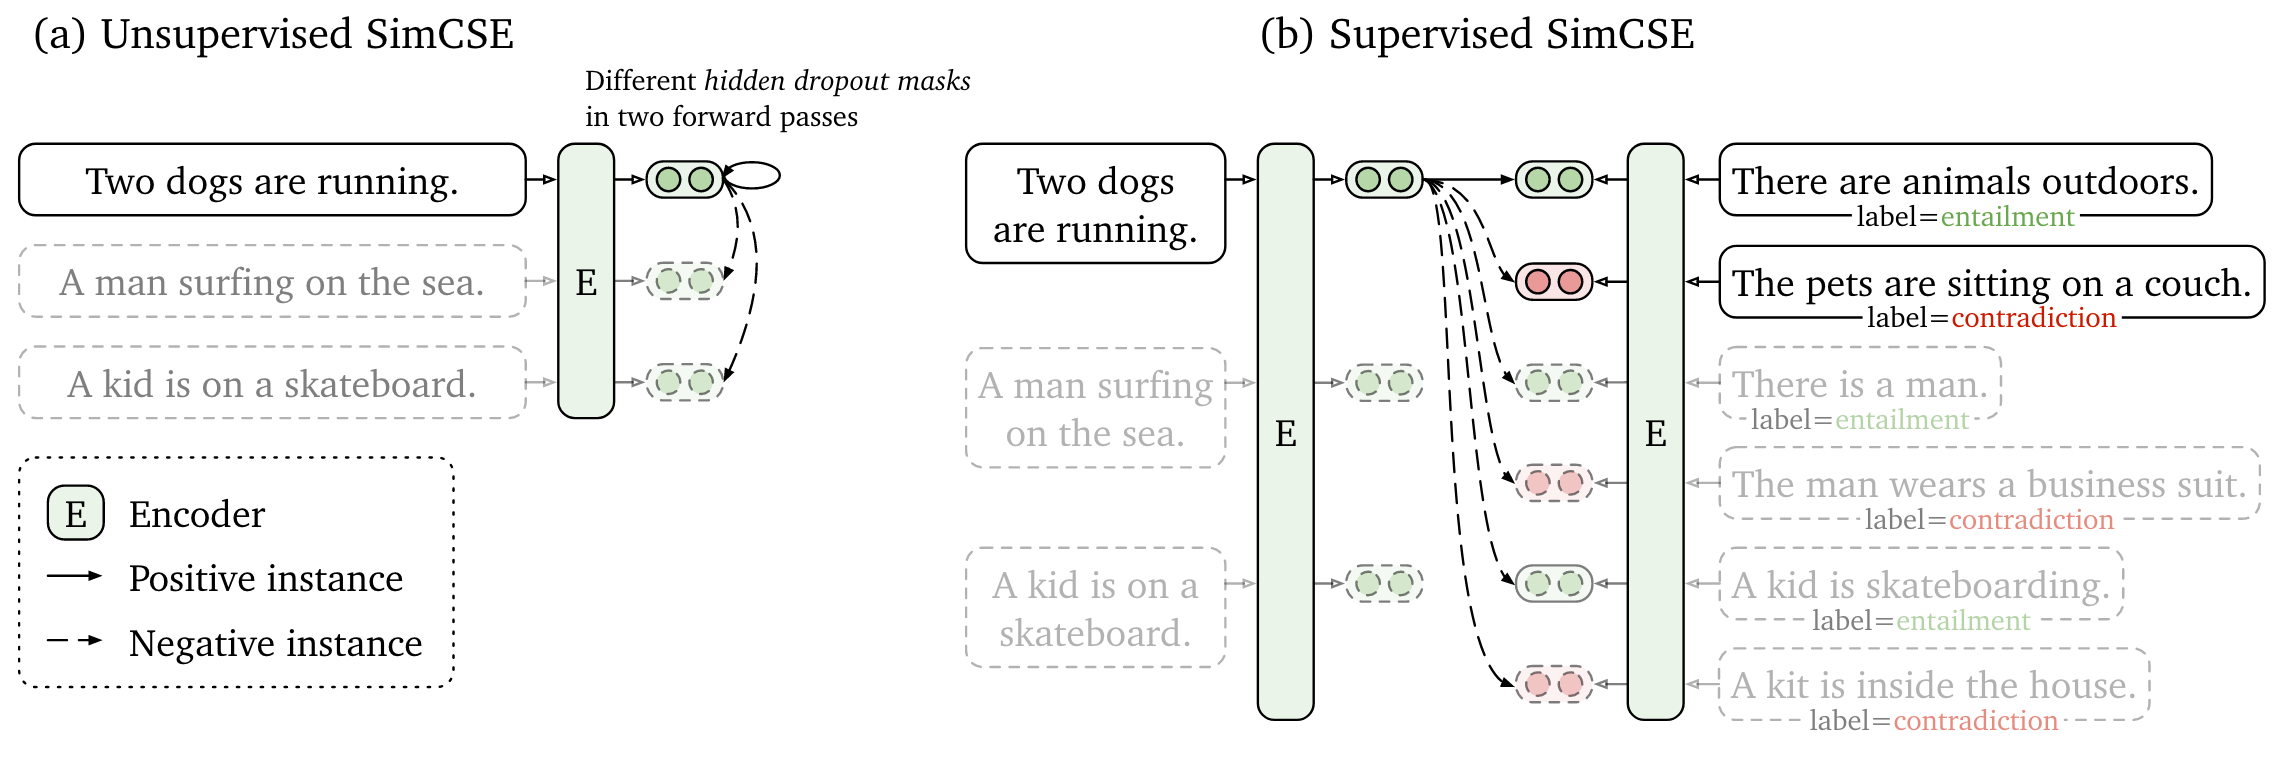
\includegraphics[width=10.0cm]{figs/SimCSE.png}}
	\caption{General idea of SimCSE.}
	\label{fig:SimCSE}
\end{figure}

SimCSE~\mycite{gao2021simcse} (Simple Contrastive Learning of Sentence Embeddings) leverages the dropout mask (like in BERT) to achieve the positve sample pairs, and proposes a supervised SimCSE w/ a natural language inference (NLI) datasets.
In the dataset, each sentence (aka., query) contains one entailment and one contradication.
The entailment is the positive sample (aka., key), the contradiction is the negative sample (key).
According to Want et al.~\mycite{wang2020hypersphere}, the quality of contrastive learning can be measured by alignment (the distance of the latent representations of the positive pair should close) and uniformity (the distance of the query and all the negative keys should scatter uniformly on the hypersphere).
It's shown~\mycite{wang2020hypersphere} that the anisotropy problem appears in language representations.
The number of (dominating and significant) singular values of the word embedding matrix in a language model decay drastically.
This is unfavorable to the uniformity.

ELECTRA~\mycite{clark2020electra} utilizes a GAN-style training process to learn a more powerful LM.
It uses MLM (masked language modeling, e.g., BERT) as the generator.
The output of the generator replaces the masked tokens with the predicted ones.
The discriminator is also a transformer encoder, whose \emph{replaced token detection} task is to predict whether each token in the output of generator is replaced by the generator or not.
The discriminator is the final pre-trained LM and the generator is a auxiliary network.
Compared with MLM-based methods, ELECTRA substantially outperforms them with less computations.
COCO-LM~\mycite{meng2021cocolm} enhances the replaced token detection of ELECTRA with CLM (Correcting Language Modeling).
The CLM is with a multi-task setting that combines the copy mechanism (aka., replaced token detection) and (a harder task) correction of the replaced tokens.
Pretraining at token level does not explicitly learn language semantics at the sequence level.
In addition to the token level pretraining, COCO-LM also introduces a sequence contrastive learning task (SCL).
The SCL is just a vanilla contractive learning where the query is the original sequence and the positive key is the randomly cropping of the query.
The output of \texttt{[CLS]} token is used as the representation of the whole sequence.

DeCLUTR~\mycite{DeCLUTR} proposes a token-level contrastive learning task based on span sampling.
The anchor is a randomly sampled span in a document.
For each anchor, there are multiple positive spans sampled near by the anchor.
The length of the anchor is longer than it's positives.
In most cases, the positive span is overlapped or subsumed with the anchor.
The negative spans inlcude easy (sampled from other documents) and hard negatives (sampled from the same document of the anchor).
A pooler (aka., mean pooling) maps the encodings of the tokens in the sample into a fixed-length encoding.
The performance of the mean pooling outperforms the embedding of \texttt{[CLS]} token.


\subsection{Relation to Metric Learning}

Metric learning is a type of representation learning that aims to learn an embedding space where the vector representations of similar data are mapped close together, and vice versa.
As a most successful approach of deep metric learning, contrastive learning attempts to close the distance between the anchor (aka., query) data point and some corresponding positive data points.
Under the setting of metric learning, MLM can be seen as an instance of contrastive learning.

\section{Graph Neural Networks}

Types:

\begin{itemize}
	\item \textbf{Homogeneous graph}: only one type of nodes and edges.
	\item \textbf{Heterogeneous graph}: there are multiple types of nodes or edges.
	\item \textbf{Hypergraph}: degree of the edge may large than two.
\end{itemize}

GNN:

\begin{itemize}
	\item GCN
	\item GraphSAGE
	\item GAT
	\item HetGNN
	\item HGNN
\end{itemize}

Model Optimization:

\begin{itemize}
	\item (TBD)
\end{itemize}

SURGE~\mycite{SURGE} proposes a novel GNN architecture to approach sequential recommendation by taking into consideration the implicit and noisy signal behaviors and fast-changing preferences.
According to the prior assumption that neighbor nodes are similar, and dense subgraphs are the core interests of users.
The authors construct graph with metric learning.
Given two item (node) embeddings $h_i, h_j$, the multi-head similarity metric function is:

\begin{align}
	M_{ij}^\delta &= \cos(w_\delta \odot h_i, w_\delta \odot h_j), \\
	M_{ij} &= \frac{1}{\phi} \sum_{\delta = 1}^\phi M_{ij}^\delta
\end{align}
where each head can be seen as one perspective and each element in weight vector $w_\delta$ is used to adaptively highlight different dimensions of the item embeddings.

Constructing graph from the similarity matrix $M$ w/ $\epsilon$-sparseness:

\begin{equation}
	A_{ij} = \begin{cases}
		1, & M_{ij} \ge \text{Rank}_{\epsilon n^2} (M); \\
		0, & \text{otherwise};
	\end{cases}
\end{equation}
where $A$ is the adjacency matrix of the generated graph and $\text{Rank}_{\epsilon n^2}(\cdot)$ returns the value of $\epsilon n^2$-th largest value.

To gather weak (implicit) signals to strong (explicit) ones that accurately reflect user perferences, the information in the graph is aggregated (interest fusion) via cluster- and query (current target prediction item)-aware graph attentive convolution:

\begin{equation}
	h_i^\prime = \parallel_{\delta = 1}^\phi \sigma (W_a^\delta \cdot \text{Agg}(E_{ij}^\delta \cdot h_j | j \in \mathcal{N}(i)) + h_i)
\end{equation}
where $\text{Agg}(\cdot)$ is the aggregation function such as mean, sum, etc, $E_{ij}^\delta$ are normalized attention coefficients obtained by the $\delta$-th attention head, $W_a^\delta$ is a linear transformation, and $\parallel$ denotes the concatenation operation.

The cluster- and query-aware attention $E_{ij}$ (for one head) is given by:

\begin{align}
	\alpha_i &= \text{Att}_c (W_c h_i \parallel h_{i_c} \parallel W_c h_i \odot h_{i_c}), \\
	\beta_j &= \text{Att}_q (W_q h_j \parallel h_t \parallel W_q h_j \odot h_t), \\
	E_{ij} &= \text{softmax}_j (\alpha_i + \beta_j) = \frac{\exp (\alpha_i + \beta_j)}{\sum_{k \in \mathcal{N}_i} (\exp (\alpha_i + \beta_k))}
\end{align}
where $h_{i_c}$ is the average value of all nodes' embedding in the cluster ($k$-hop neighborhood) of the node $h_i$, $\text{Att}$ is a two-layer MLP w/ LeakyReLU, $h_t$ is the target (query) item embedding (\textit{viz.} learn the user interest's independent evolution for different target intertests), and $E_{ij}$ is the additive attention to consider the factors of cluster and query simultaneously.

Graph pooling is applied to fuse (aka. evolution) implicit interest signals to explicit ones.

\begin{align}
	S_{i,:} &= \text{softmax} (W_p \cdot \text{Agg} (A_{ij}) \cdot h_j^\prime | j \in \mathcal{N}_i), \\
	[h_1^*, \cdots, h_m^*] &= S^\top [h_1^\prime, \cdots, h_n^\prime]^\top, \\
	[\gamma_1^*, \cdots, \gamma_m^*] &= S^\top [\gamma_1^\prime, \cdots, \gamma_n^\prime]^\top, \\
	\gamma_i &= \text{softmax}_i (\beta_i), \\
	A^* &= S^\top A S
\end{align}
where $S \in \mathbb{R}^{n \times m}$ is a soft cluster assignment matrix.

However, it is difficult to train $S$ and the temporal order of the nodes $h_i$ and the pooled nodes $h_i^*$ reflect the historical user interest.
The authors use some trivial regularization terms to alleviate the issue.

\begin{align}
	L_M = \lVert A - SS^\top \rVert_F, \quad &\parbox{15em}{ make two nodes with greater connection strength map to the same cluster}, \\
	L_A = \frac{1}{n} \sum_{i=1}^n H(S_{i,:}), \quad &\parbox{15em}{ approach rach row a one-hot vector}, \\
	L_P = \lVert p_n S - p_m \rVert_2, \quad &\parbox{15em}{ make the position of the non-zero elements in S closer to the main diagonal elements}
\end{align}
where position encoding vectors $p_n = [1, 2, \cdots, n], p_m = [1, 2, \cdots, m]$.

Graph readout to aggregates all node embeddings of the raw graph (before pooling):

\begin{align}
	h_g = \text{Readout} ([\gamma_i \cdot h^\prime_i | i \in \mathcal{G}])
\end{align}
where $\text{Readout}(\cdot)$ is just the sum in the paper to ensure permutation invariant.

Any sequential recommendation method can be used to model the pooled sequence $h^*$, where this paper uses $h_s = \text{AUGRU}(h_1^*, \cdots, h_m^*)$.
The final prediction is:

\begin{equation}
	\hat{y} = \text{Pred} (h_s \parallel h_g \parallel h_t \parallel h_g \odot h_t)
\end{equation}
where Pred is a two-layer MLP.

The task is CTR (CTR).
The loss is vanilla NLL (negative log-likelihood) w/ L2 regularization term.

LightGCN~\mycite{lightgcn} conducts extensive ablation studies on NGCF and finds that feature transformation and nonlinear activation of GCN contribute little and even negatively to collaborative filtering.
For NGCF~\mycite{NGCF} (Neural Graph Collaborative Filtering), given the ID embedding $e_u^{(0)}$ of user $u$ and $e_i^{(0)}$ of item $i$, the outputs of the layer $(k+1)$ are:

\begin{align}
	e_u^{(k+1)} &= \sigma\left( W_1 e_u^{(k)} + \sum_{i \in \mathcal{N}_u} \frac{1}{\sqrt{|\mathcal{N}_u||\mathcal{N}_i|}} (W_1 e_i^{(k)} + W_2(e_i^{(k)} \odot e_u^{(k)})) \right), \nonumber \\
	e_i^{(k+1)} &= \sigma\left( W_1 e_i^{(k)} + \sum_{u \in \mathcal{N}_i} \frac{1}{\sqrt{|\mathcal{N}_u||\mathcal{N}_i|}} (W_1 e_u^{(k)} + W_2(e_u^{(k)} \odot e_i^{(k)})) \right) \label{eq:NGCF}
\end{align}
where $\mathcal{N}_i$ denotes the set of users that interact with item $i$, $\mathcal{N}_u$ denotes the set of items that are interacted by user $u$.

The above formula~\ref{eq:NGCF}'s matrix form is implemented with graph Laplacian (exact the one used in GCN~\mycite{GCN}):

\begin{align}
	E^{(k+1)} &= \sigma \left( (I + \mathcal{L}) E^{(k)} W_1 + (\mathcal{L} E^{(k)}) \odot E^{(k)} W_2 \right), \\
	\mathcal{L} &= D^{-\frac{1}{2}} A D^{-\frac{1}{2}}
\end{align}
where $A$ is the adjacency matrix and $D$ is the diagonal degree matrix (w/ some tricks mentioned in GCN).

NGCF then concatenates the embeddings of all layers to obtain the final user and item embeddings, using the inner product to generate the prediction score.

The authors of LightGCN argue that the nodes in tasks of the original GCN paper have rich semantic features such as the title and the abstract, but in collaborative filtering, each node only has an ID.
The motivation of LightGCN is very reasonable and the story is nice.
The LGC (Light Graph Convolution) at layer $k$ is defined as:

\begin{align}
	e_u^{(k+1)} &= \sum_{i \in \mathcal{N}_u} \frac{1}{\sqrt{|\mathcal{N}_u||\mathcal{N}_i|}} e_i^{(k)}, \\
	e_i^{(k+1)} &= \sum_{u \in \mathcal{N}_i} \frac{1}{\sqrt{|\mathcal{N}_u||\mathcal{N}_i|}} e_u^{(k)}
\end{align}

The final embeddings are (learnable) weighted sum of the outputs of all layers:

\begin{align}
	e_u &= \sum_{k=0}^K \alpha_k e_u^{(k)}, e_i = \sum_{k=0}^K \alpha_k e_i^{(k)}, \\
	\hat{y}_{u,i} &= e_u^\top e_i
\end{align}

LightGCN employs Bayesian Personalized Ranking (BPR) loss that encourages the prediction of an observed entry to behigher than its unobserved counterparts:

\begin{equation}
	\mathcal{L} = - \sum_{u=1}^M \sum_{i \in \mathcal{N}_u} \sum_{j \ne \mathcal{N}_u} \ln \sigma (\hat{y}_{u,i} - \hat{y}_{u,j}) + \lambda \lVert E^{(0)} \rVert^2
\end{equation}

For user and item attribute (e.g., Female is a user attribute, sci-fi is a item attribute for a moive) interactions, there are two types of attributes interactions: inner interactions (interactions between homogeneous attributes, aka. both user or both item attributes), cross interactions (between heterogenous attributes).
Existing methods do not distinguish these two types of interactions.
GMCF~\mycite{GMCF} (Neural Graph Matching based Collaborative Filtering) aruges that it is most effective way to explicitly model these two types of interactions separately.

Formally, user attributes and item attributes are both the set of key-value pairs (e.g., \texttt{(female, 1)}, \texttt{(age, 22)}).
Each node is the embedding of the attribute $u = \text{val} \cdot e_{\text{attribute}}$.
User attribute graph is a \concept{complete} graph constructed from attributes of the user, which is same as the item attribute graph.

The inner interaction (for characteristic learning) is just the edge between two nodes in the same graph and is modeled by a MLP.
After message passing, the new representation of node $i$ is $z_i = \sum_{j \in \mathcal{N}(i)} \text{MLP}_{2d \rightarrow d} (u_i \parallel u_j)$.

The cross interaction (for node matching) is modeled by Hadamand product between the node of user graph and the node of item graph.
The node matching result is the aggregation of a node in one graph and all node in the other graph: $s_i^U = \sum_{j \in V(I)} u_i^U \odot u_j^I$.

The final node representation is fused by GRU with the input sequence $[u_i, z_i, s_i]$.
The final graph representations are $v_G^U = \sum_{i \in V(U)} u_i^U, v_G^I = \sum_{i \in V(I)} u_i^I$.
The task is the prediction of an action (e.g., watch, like) w.r.t. a user and an item, using the inner product (graph matching) of user graph and item graph: $\hat{y} = v_G^{U \top} v_G^I$.

In overall, the motivation to distinguish two types of interactions is reasonable and gains some improved performance.
However, the proposed two graphs cannot bring any structure information (i.e., the edge information) of the graph because they are complete graphs.
The fusion part (GRU over a sequence of three elements) is a unreasonable and stiff hyperparameter tuning.
Besides, this work lacks the usage of the information of the relation between users and the historical interactions of the user.
According to the ablation experiments (Fig. 3 and Table 3), the fusing algorithm ($\text{MLP} \rightarrow \text{GRU}$ improves 0.0102 AUC) contributes more than using different interactions ($\texttt{<Bi, Bi>} \rightarrow \texttt{<MLP, Bi>}$ improves 0.0093 AUC).

Multi-behavior recommendation: given a user and an item, there are multiple behavior types (aka., interactions, e.g., view, purchase, favorite) between them.
HMG-CR~\mycite{HMG-CR} (Hyper Meta-Graph Contrastive learning for Recommendations) proposes hyper meta-graph contrastive learning to learn the encoder for each behavior that awares other bahaviors.
For each user $u_i$ and behavior $r_j$, the user and all items she interacted are constructed to a hyper meta graph $\mathcal{G}_j^i$.
I think this hyper meta graph is not actual "hyper" like hypergraph.
For each behavior we will have different graph encoder (aka., the parameters are not shared) $h_j^i = g_t (\mathcal{G}_j^i)$.
To leverage constrative learning, the negative pair is $(h_{j-1}^i, h_j^i)$ and the positive is $h_j^i$ and $\hat{h}^i_j = g_{j-1} (\mathcal{G}_j^i)$.
Another training task is recommendation task, where we need predict the interaction between the user (represented as the fusion of all encodings of the hyper meta graphs) and a given item.

For session-based recommendation (SBR), there are many sessions for one user.
Each session (e.g., item1 => item2 => item3 => item2 => item4) can be constructed into a (session) weighted graph.
Because the node (item) set in all the session graphs are same.
Besides the session graph, GCE-GNN~\mycite{wang2020global} (Global Context Enhanced Graph Neural Networks) proposes a global graph that combines all the sessions.
Based on GCE-GNN, DAT-MDI (dual attention transfer based on multi-dimensional integration)~\mycite{dat-mdi} enhances it with multi-domain scenario.
According to the Section 1 in the paper, different domain has different items.
The assumption is that if two users have similar session behaviour in one domain (e.g., view), they should have similar session behaviour in another domain (e.g., click or purchase).
Conceptually, the multi-domain is like multi-behaviour but can be more general.
The authors proposes a dual attention transfer learning layer to learn better item representations by considering the relation of the similarity across domains.
However, the formula (most of them are borrowed from GCE-GNN) in this paper has so many mistakes.
And it seems consume far more computing resources than GCE-GNN (but no experiments given).

SBR also suffers from the very long behavior history.
Current industrial solutions that truncate the sequences will leads modelings periodicity or long-term dependency a problem.
In UBR4CTR~\mycite{UBR2CTR} (User Behavior Retrieval for CTR prediction), the most relevant and appropriate user behaviors will be firstly retrieved from the entire user history sequence using a learnable search method.
Given the user behavior history $H_u = {b_1^u, \cdots, b_T^u}$ for user $u$, each behavior is consist of user features $u = [ f_1^u, \cdots, f_{K_u}^u ]$, item features $v = [f_1^v, \cdots, f_{K_v}^v]$, and context (e.g., time and scenario) feature $c = [f_1^c, \cdots, f_{K_c}^c]$.
The input of each behavior is the embeddings of it's categorical field features: $b_i^u \in \mathbb{R}^{K \times d} = u \parallel v \parallel c$.
UBR4CTR contains user behavior retrieval and prediction module. 
For user behavior retrieval, the query is $q = u \parallel v \parallel c$ and UBR4CTR utilizes self-attention to randomly select subset of features w/ the probability $\hat{E} = \text{sigmoid}(\text{MLP}(\text{Multihead}(q, q, q))) \in \mathbb{R}^K$, where $q \in \mathbb{R}^{K \times d}$.
The similarity between $q = [f_1, \cdots, f_n]$ after randomly selecting and all the history behaviors $H_u$ can be seen as searching one sentence in the document sorted by the number of matched words.
The behavior search is based on SM25 (similar to TF-IDF) and can be seen as searching for exact match fields:

\begin{align}
	s = \sum_{i=1}^n \log \frac{(N - N(f_i) + 0.5) (\text{TF}(f_i, H_u) \cdot 2.2)}{(N(f_i) + 0.5) (\text{TF}(f_i, H_u) + 1.2)}
\end{align}
where $\text{TF}(f_i, H_u)$ is the term frequent in $H_u$ (e.g., $f_i$ is a categorical feature representing age), $N(f_i)$ is the total number of the behaviors in $H_u$ that contains $f_i$.

According to the similarity score, we get $S$ behaviors from the very long history and use a simple soft attention with MLP to perform CTR.
Because the history behavior search is indifferentiable, reinforcement learning \concept{($\pi_{\theta} (H_u^{(S)}) = \prod_{j=1}^n p(f_j)$, just expand the expectation of the loss, use log-trick, and approximate the distribution $\pi$ as the empirical distribution)} is used to train the model.
However, the behavior retrieval proposed by UBR4CTR is based on exact matching which misses the semantic similarity between the categorical features (e.g., T-shirts is close to pants).

\sidenotedcmmc{log-trick: \url{https://medium.com/@aminamollaysa/policy-gradients-and-log-derivative-trick-4aad962e43e0}}

Alibaba solve the very long ($\ge 54,000$ and get $7.1\%$ CTR lifting in Alibaba display advertising system) history behavior problem with a search-based interest model (SIM~\mycite{SIM}).
For a given target item (aka., query) $a$, the relevant score is:

\begin{equation}
	r_i = \begin{cases}
		\text{sign} (C_i = C_a), &\text{hard-search;} \\
		(W_b e_i) (W_a e_a)^\top, &\text{soft-search;}
	\end{cases}
\end{equation}
where for the soft-search, directly using the parameters learned from short-term user interest modeling in soft-search model may mislead the long-term user interest modeling.
So, the authors train the soft-search model (inner product plus a MLP) under an auxiliary CTR prediction task based on long-term behavior data.

According to the relevant scores, the top-K related sub-user behavior sequence $B^*$ is selected from long-term user behaviors.
The input feature of the history behavior is concatenated with the embedding of time intervals.
And the precition model is based on $\text{Multihead}(e_a, B^*, B^*)$.
External features and other sequential model (e.g., DIEN) can also be added.
